\begin{figure}[H]
    \centering
    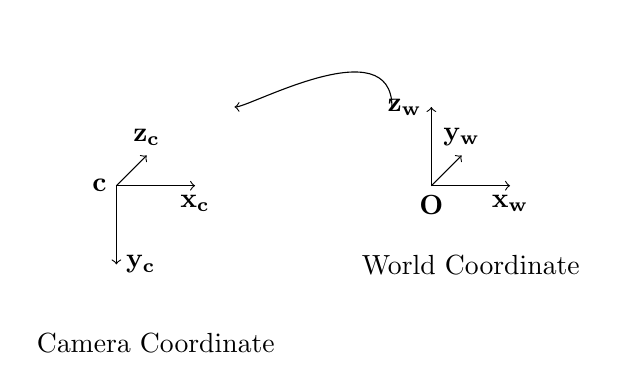
\begin{tikzpicture}[->]
        \begin{scope}[xshift=3.5cm]
            \draw (0,0,0) -- (xyz cs:x=1)node[below]{$\bf{x}_w$};
            \draw (0,0,0) -- (xyz cs:y=1)node[left]{$\bf{z}_w$};
            \draw (0,0,0) -- (xyz cs:z=-1)node[above]{$\bf{y}_w$};
            \node (O) at (0,0,0) [below] {$\bf{O}$};
        \end{scope}
        \draw[->] (3,1) .. controls +(up:1cm) and +(right:0.2cm) .. (1, 1);
        \begin{scope}[xshift=-0.5cm]
            \draw (0,0,0) -- (xyz cs:x=1)node[below]{$\bf{x}_c$};
            \draw (0,0,0) -- (xyz cs:y=-1)node[right]{$\bf{y}_c$};
            \draw (0,0,0) -- (xyz cs:z=-1)node[above]{$\bf{z}_c$};
            \node (P) at (0,0,0) [left] {$\bf{c}$};
        \end{scope}
        \node (A) at (0, -2) {Camera Coordinate};
        \node (B) at (4, -1) {World Coordinate};
    \end{tikzpicture}
    \caption{FlipY Camera Model}
    \label{fig:flip_y_camera}
\end{figure}